% !TEX TS-program = XeLaTeX

% STYLE

\documentclass[a4paper, 12pt]{article}
\usepackage[left=3cm,
		    right=3cm,
    		    top=3cm,
		    bottom=3cm,
		    bindingoffset=0cm]{geometry}
		    \usepackage{array}
\usepackage{float}
\usepackage{graphicx}
\usepackage{hyperref}
\hypersetup{
    colorlinks=true,
    linkcolor=black,
    citecolor=black,
    filecolor=black,
    urlcolor=black,
}
\graphicspath{ {./images/} }
\usepackage{subfig}
%\usepackage{enumerate}
\usepackage[normalem]{ulem} % underlining
\usepackage{booktabs} % tables
\PassOptionsToPackage{table}{xcolor}% coloring tables
\usepackage[shortlabels]{enumitem}
\setlist[enumerate]{itemsep=-3pt}

% LANGUAGE + FONT
		    
\usepackage[english]{babel}
\usepackage[backend=biber,
                     style=unified]{biblatex}
\newcommand{\citeay}[2][]{
   \citeauthor{#2} (\citeyear[#1]{#2})}
\addbibresource{ref.bib}
\usepackage{fontspec}  
\usepackage{pifont}
\setmainfont{Minion 3}

% DRAWING

\usepackage{tikz}
\usepackage{tikz-qtree}
\usetikzlibrary{shapes.geometric}
\usetikzlibrary{trees,arrows}
\usetikzlibrary{positioning}
\usetikzlibrary{matrix}
\usetikzlibrary{tikzmark}
\usetikzlibrary{decorations.shapes}
\usetikzlibrary{shapes.misc}

% LINGUISTICS 

%\usepackage{gb4e}
\usepackage{expex}
\usepackage[glossaries]{leipzig}
\makeglossaries
%\newleipzig {indef} {indef} {Indefinite}

\title{Stress as empty CV \\ {\normalsize Phonetic and phonological exponents of stress}}
\author{Sasha Shikunova}
\date{EGG2023, last updated \today}

\begin{document}

\maketitle

%- Two levels: syllable structure and melody with a potential to associate
%- Technicalities: government, licensing, representation of syllable weight and vowel/consonant length by 2 nuclei
%- CV as an exponent of stress (Ségéral & Scheer 2008)
%- Advantages of collapsing length and stress: case studies from Italian (Larsen 1998), Saami (Enguehard 2014) or Moksha (might save it for the Uralic phonology class)
%- Summary of stress-related phenomena: vowel lengthening, consonant lengthening, aspiration, glottalization and tones
%- How the paucity of stress-related phenomena is explained in OT (Giavazzi 2010)
%- Exponents of stress: summary of diagnostics for when stress-as-length makes sense

		\section{Phonetic realisation of stress}
		
	What is a stressed syllable like?
	
	\pex
		Native speakers and phoneticians usually find it easy to determine which syllables bear stress, and even to distinguish varying degrees of stress, but the phonetic characterization of stress is exceedingly difficult: stress is variously associated with
		\begin{enumerate}[\ding{170}, labelindent=2cm, leftmargin=*]
			\item \emph{greater loudness,}
			\item \emph{higher pitch,} 
			\item and \emph{greater duration}, any of which may be most important in a given case, 
			\item and sometimes also with \emph{vowel quality}. \trailingcitation{\parencite[p. 336]{trask1996}}
		\end{enumerate}
	\xe
%	(examples)

			\subsection{Stress-related phenomena}
			
	There is a limited range of phenomena that are conditioned by stress, as argued by \textcite{giavazzi2010}
	
	\ex
		It is surprising fact that a large number of phonological features never participate in stress-conditioned processes. \trailingcitation{\parencite[p. 12]{giavazzi2010}}
	\xe
	
	\begin{enumerate}[$\gg$]
		\item the preservation or neutralisation of segmental contrast in the vicinity of stress
	\pex In Italian, [k] is preserved next to stressed vowels
		\a /an.'ti.k-i/ [an.(ti)\textsubscript{{\'σ}}.ki] 'antique', Masc. Pl. 
		\a /'ko.mi.k-i/ [(ko)\textsubscript{{\'σ}}.mi.tʃi] 'comic', Masc. Pl. \trailingcitation{\parencite[p. 13]{giavazzi2010}}
	\xe
		\item the enhancement of the acoustic properties of the releases in stress-adjacent consonants (e.g. affrication, aspiration)
	\pex In English, initial and pre-stress voiceless stops are aspirated
		\a \emph{pay} [p\textsuperscript{h}eɪ]
		\a \emph{spare} [speə\textsuperscript{r}]
		\a \emph{potato} [p\textsuperscript{h}ət\textsuperscript{h}eɾo]
	\xe
	
	\pex~ In Southern Saami, codas of stressed syllables are preaspirated/geminated
		\begin{figure}[H]
			\centering
			\includegraphics[width=.9\textwidth]{enguehard2014}
		\end{figure}
		\trailingcitation{\parencite{enguehard2014}}
	\xe
	\end{enumerate}
	There is a phonetically grounded way of explaining why only certain features can be affected by the vicinity of stress. It is because of the characteristic exponents of stress: duration and loudness (loudness is followed by increased subglottal pressure which affects articulation of stops). 

		\section{Phonological exponence}
		
	Can stress be a feature? Suppose [stress] feature exists:
	
	\begin{enumerate}[$\gg$]
		\item Stress can easily be lexically encoded
		\item In OT, there is now no problem with implementing prosodic structure in the input \parencite{delacy2019}
		\item (contrastive syllabification should not be possible)
	\end{enumerate}
	But:
	
	\begin{enumerate}[$\gg$]
		\item The feature [stress] would be characterised by \textsc{obligatoriness} and \textsc{culminativity}
		\item Is it true of any other feature?
		\item How many values should [stress] have? There is primary and secondary stress
	\end{enumerate}
	
	\noindent [Stress] is different from other SPE features (\cite[pp. 262--263]{liberman-prince1977} as summarised by \cite[pp. 208]{roca1994}):
	
	\renewcommand{\arraystretch}{1.2}
\begin{table}[H]
\centering
\begin{tabular}{ll}
\toprule
Stress                   & Other DFS               \\
\midrule
n-ary valency            & binary valency          \\
syntagmatic definition   & paradigmatic definition \\
global effects           & local effects           \\
derivationally preserved & derivationally affected \\
disjunctive application  & conjunctive application \\
\bottomrule
\end{tabular}
\end{table}
	
	\noindent What should stress be, if not a feature?
	
	\begin{enumerate}[$\gg$]
		\item Be lexically encodable
		\item Sensibly correspond to duration, loudness and/or pitch
		\item Be responsible for the fortition effects around it
	\end{enumerate}
	
%	The existence of [stress] is convenient in Optimality Theory, where the prosodic structure is not welcome in the input, but if there exists a stress assignment algorithm that determines the stress placement and inserts an exponent, then what should it be, if not a feature?

		\section{A flat two-tiered phonology}
		
	\begin{enumerate}[$\gg$]
		\item Strict CV (also CVCV) is a lateral autosegmental theory of phonology \parencite{klv1990, scheer2012}
		\item Two tiers: syllabic and melodic
		\item Uniform syllable structure -- CV
		\item Melody associated to the syllabic skeleton or floating
	\end{enumerate}
	Two opposite lateral forces: government and licensing (since Government phonology). Government decreases the prominence of a segment, whereas licensing increases it.
	
	\pex
		\textbf{Proper Government (PG)}
			\a PG is a form of internuclear Government 
			\a the governor may not itself be governed 
			\a PG cannot apply over a governing domain	\trailingcitation{\parencite{klv1990}}
	\xe

	\ex~
		\textbf{Licensing}: only ungoverned nuclei can license
	\xe
	
	\begin{figure}[H]
	\centering
				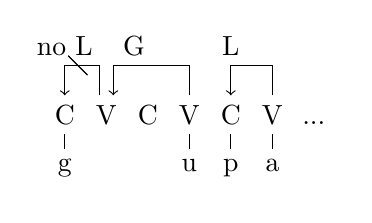
\begin{tikzpicture}
\matrix [matrix of nodes, row sep=0.1em,
column sep={1.5em,between origins}]
{
|(c2)|{C} & |(v2)|{V} & |(c3)|{C} & |(v3)|{V} & |(c4)|{C} & |(v4)|{V} & {...}     \\[0.5em]
|(C2)|{g} & |(V2)|{ } & |(C3)|{ } & |(V3)|{u} & |(C4)|{p} & |(V4)|{a} & \\
};
\draw (v3.south) -- (V3.north);
\draw (c4.south) -- (C4.north);
\draw (v4.south) -- (V4.north);
\draw (c2.south) -- (C2.north);
\draw [->] (v3.north) -- ++(north:2.5ex) -| (v2.70) node[midway,above right] {G};
\draw [->] (v2.110) -- ++(north:2.5ex) -| (c2.north) node[midway,above]  {no L} node[pos=0.3,sloped,rotate=45]{$|$}node[pos=0.3,sloped,rotate=45]{$|$};
\draw [->] (v4.north) -- ++(north:2.5ex) -| (c4.north) node[midway,above]  {L};
				\end{tikzpicture}
	\end{figure}

	Important consequence of the universal CV syllable structure and government \& licensing: the post-coda position and the initial position are the strongest, i.e. not inhibited by government and licensed at the same time \parencite{segeral-scheer2008}.
	
	\begin{figure}[H]
		\includegraphics[width=\textwidth]{strongs}
	\end{figure}
		
	\begin{figure}[H]
		\includegraphics[width=\textwidth]{weaks}
	\end{figure}
	
	\hfill \parencite[p. 490]{segeral-scheer2008}	\\
	
	\noindent One major way of representing stress in CVCV is an empty skeletal unit -- empty CV \parencite{larsen1998, scheersszigetvari2005, enguehard2015}.
	
			\begin{minipage}{0.4\linewidth}
			\ex {[fa:to]} (Italian) \\
				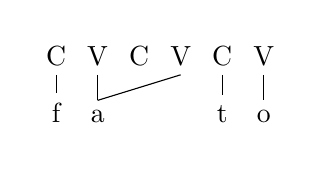
\begin{tikzpicture}
\matrix [matrix of nodes, row sep=0.1em,
column sep={1.5em,between origins}]
{
|(c1)|{C} & |(v1)|{V} & |(c2)|{C} & |(v2)|{V} & |(c3)|{C} & |(v3)|{V}      \\[0.6em]
|(C1)|{f} & |(V1)|{a} & |(C2)|{} & |(V2)|{} & |(C3)|{t} & |(V3)|{o} \\
};
\draw (c1.south) -- (C1.north);
\draw (v1.south) -- (V1.north);
\draw (c3.south) -- (C3.north);
\draw (v2.south) -- (V1.north);
\draw (v3.south) -- (V3.north);
				\end{tikzpicture}
			\xe
		\end{minipage}
		\hfill
		\begin{minipage}{0.5\linewidth}
			\ex {[rip\textsuperscript{h}i:t]} (English)\\
				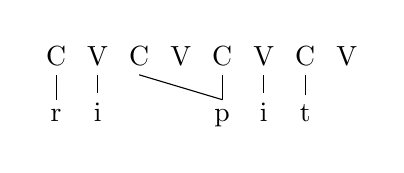
\begin{tikzpicture}
\matrix [matrix of nodes, row sep=0.1em,
column sep={1.5em,between origins}]
{
|(c1)|{C} & |(v1)|{V} & |(c2)|{C} & |(v2)|{V} & |(c3)|{C} & |(v3)|{V}  & |(c4)|{C} & |(v4)|{V}      \\[0.6em]
|(C1)|{r} & |(V1)|{i} & |(C2)|{} & |(V2)|{} & |(C3)|{p} & |(V3)|{i} & |(C4)|{t} & |(V4)|{} \\
};
\draw (c1.south) -- (C1.north);
\draw (v1.south) -- (V1.north);
\draw (c2.south) -- (C3.north);
\draw (c3.south) -- (C3.north);
\draw (v3.south) -- (V3.north);
\draw (c4.south) -- (C4.north);
				\end{tikzpicture}
			\xe
		\end{minipage}
	The effects of the empty CV depend on whether it is inserted to the right or to the left of the stressed syllable:
	
	\begin{enumerate}[$\gg$]
		\item The CV inserted to the right lengthens the stressed vowel (Italian)
		\\$\Rightarrow$ stressed syllables are heavy 
		\item The CV is inserted to the left fortifies the onset of the stressed syllable (English)
		\\$\Rightarrow$ onsets of stressed syllables are strong
	\end{enumerate}
	This way, fortition in stress-adjacent position is linked to fortition in strong positions. Stress as a property of vowels is linked to length. Also, weight-sensitivity of stress can be parametrised in the CVCV system:
	
	\begin{enumerate}[$\gg$]
		\item Universal syllable structure
		\\$\Rightarrow$ CVC syllables are actually CVCØ 
		\item Parametrised projection of empty nuclei
		\\$\Rightarrow$ languages may or may not be weight-sensitive
	\end{enumerate}

			\subsection{Case studies}
		
	\citeay{enguehard2014} proposes a modification of the empty CV analysis of stress for the Southern Saami language -- a CV unit with the element h\textsuperscript{0}, which is responsible for pre-aspiration.
	
	\begin{enumerate}[$\gg$]
		\item Southern Saami has fixed initial stress
		\item Initial stressed syllables ``can have the structures (C)VC, (C)VV, (C)VVC, but never *(C)V'' \parencite[p. 49]{enguehard2014}
		
	\begin{figure}[H]
		\centering
		\includegraphics[width=.9\textwidth]{enguehard2014-49}
	\end{figure} \vspace*{-2em}\hfill \parencite[p. 49]{enguehard2014}\\
		\item The stressed syllable does not just have to be heavy -- it always becomes heavier when stressed, even if it is already CVC
		\item Hence the insertion of the CV
	\end{enumerate}

	\begin{figure}[H]
%		\centering
		\includegraphics[width=.6\textwidth]{enguehard2014-54a}
	\end{figure}
	
	\begin{figure}[H]
%		\centering
		\includegraphics[width=.8\textwidth]{enguehard2014-54b}
		\\ \hfill \parencite[p. 54]{enguehard2014}
	\end{figure}
			
		\section{Summary}
		
	\begin{enumerate}[$\gg$]
		\item Empty CV as an exponent of stress can account for both weight-sensitive and weight-independent stress systems
		\item Fortition effects around stress receive the same explanation as the strength of the Coda disjunction -- {\#\_/C\_}
		\item Can be modified to include other elements
	\end{enumerate}
	
			\subsection{Next up...}
			
	CVCV meets metrical grids -- Strict CV Metrics:
	
	\begin{enumerate}[$\gg$]
		\item Mechanisms targeting grid marks: projection and incorporation
		\item Parametrisation: which nuclei do and do not project?
		\item How sophisticated weight hierarchies can be modelled with the universal CV syllable structure
	\end{enumerate}
		
\printbibliography
\end{document}